\begin{name}
	{\tenchude}
	{\tendethi}
	{Chuyên ĐH Vinh L1 2021-2022}
	{\thoigian}
\end{name}
\Opensolutionfile{ans}[ans/ans-2-TT-ChuyenDH-Vinh-L1-NH21-22]
	%%==========Câu 1
\begin{ex}%[2D3Y1-1]
	Cho hàm số $f(x)=x^3-2x$. Khẳng định nào sau đây đúng?
	\choice
	{$\displaystyle\int f(x)\mathrm{\,d}x=\dfrac{x^4}{4}+x^2+C$}
	{ $\displaystyle\int f(x)\mathrm{\,d}x=x^4-x^2+C$}
	{$\displaystyle\int f(x)\mathrm{\,d}x=3x^2-2x+C$}
	{\True $\displaystyle\int f(x)\mathrm{\,d}x=\dfrac{x^4}{4}-x^2+C$}
	\loigiai{
		Ta có $\displaystyle\int f(x)\mathrm{\,d}x=\displaystyle\int (x^3-2x)\mathrm{\,d}x=\dfrac{x^4}{4}-x^2+C$.
	}
\end{ex}
%%==========Câu 2
\begin{ex}%[2D2Y4-1]
	Tập xác định của hàm số $y=\log_{3}(2-x)$ là
	\choice
	{$[0;+\infty)$}
	{$(0;+\infty)$}
	{$\mathbb{R}$}
	{\True $(-\infty;2)$}
	\loigiai{
		Điều kiện xác định $2-x>0 \Leftrightarrow x<2$.\\
		Tập xác định $\mathscr{D}=(-\infty;2)$.
	}
\end{ex}
%%==========Câu 3
\begin{ex}%[2D1Y4-1]
	Cho hàm số $y=f(x)$ có bảng biến thiên
	\begin{center}
		
\begin{tikzpicture}[>=stealth]
		\tkzTabInit[nocadre=true,lgt=1.2,espcl=3,deltacl=0.5]{$x$/.7 ,$f'(x)$/.7,$f(x)$/2}
		{$-\infty$ , $1$ , $+\infty$}
		\tkzTabLine{ , + , d , + , }
		\tkzTabVar{-/$-1$ , +D-/$+\infty$/$-\infty$ , +/$-1$}
		\end{tikzpicture}
	\end{center}
	Số đường tiệm cận của hàm số đã cho là
	\choice
	{$4$}
	{\True $2$}
	{ $3$}
	{$1$}
	\loigiai{
		Tập xác định $\mathscr{D}=\mathbb{R}\backslash \{1\}$.\\
		Ta có\\
		\qquad $\lim\limits_{x\to +\infty}f(x)=-1$ suy ra $y=-1$ là tiệm cận ngang.\\
		\qquad $\lim\limits_{x\to -\infty}f(x)=-1$ suy ra $y=-1$ là tiệm cận ngang.\\
		\qquad $\lim\limits_{x\to 1^{-}}f(x)=+\infty$ suy ra $x=1$ là tiệm cận đứng.
	}
\end{ex}
%%==========Câu 4
\begin{ex}%[2D1Y1-2]
	\immini
	{Cho hàm số $y=f(x)$ có đồ thị như hình vẽ. Hàm số đồng biến trên khoảng nào trong các khoảng sau?
		\choice
		{$(-2;2)$}
		{$(2;+\infty)$}
		{\True $(0;2)$}
		{$(-\infty;0)$}}
	{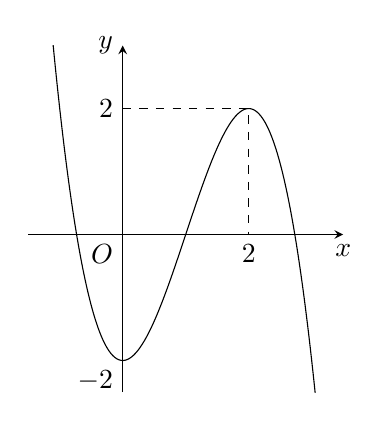
\begin{tikzpicture}[>=stealth,x=1cm,y=1cm,scale=0.8]
		\def\a{-1}
		\def\b{3}
		\def\c{0}
		\def\d{-2}
		\draw[->] (-1.5,0) -- (3.5,0)node[below]{$x$};
		\draw[->] (0,-2.5) -- (0,3) node[left] {$y$};
		\draw (0,0)node[below left]{$O$};
		\draw (2,0)node[below]{$2$};
		\draw (0,-2)node[below left]{$-2$};
		\draw (0,2)node[left]{$2$};
		\clip (-1.5,-2.5)rectangle(3.5,3);
		\draw[samples=150,smooth,domain=-1.5:3.5] plot(\x,{\a*(\x)^3+(\b)*(\x)^2+(\c)*\x+(\d)});
		\draw[dashed] (0,2)--(2,2)--(2,0);
		\end{tikzpicture}
	}
	\loigiai{
		Dựa vào đồ thị, hàm số đồng biến trên $(0;2)$.
	}
\end{ex}
%%==========Câu 5
\begin{ex}%[2H1Y3-2]
	Thể tích khối hộp chữ nhật có các kích thước $2$, $3$, $4$ là
	\choice
	{$6$}
	{$8$}
	{$72$}
	{\True $24$}
	\loigiai{
		Ta có $V=2\cdot 3\cdot 4=24$.
	}
\end{ex}
%Câu 6
\begin{ex}%[Huỳnh Đức Vũ]%[Thi thử Chuyên ĐH Vinh-lần 1-2022]%[2H3Y1-1]
	Trong không gian $O x y z$, toạ độ hình chiếu vuông góc của $A(4 ;-3 ; 2)$ lên trục $O z$ là
	\choice
	{ \True $(0 ; 0 ; 2)$}
	{ $(4 ;-3 ; 0)$}
	{ $(4 ; 0 ; 0)$}
	{ $(0 ;-3 ; 0)$}
	\loigiai{Toạ độ hình chiếu vuông góc của $A(4 ;-3 ; 2)$ lên trục $O z$ là $(0 ;0 ; 2)$.}
\end{ex}
%Câu 7
\begin{ex}%[Huỳnh Đức Vũ]%[Thi thử Chuyên ĐH Vinh-lần 1-2022]%[1D2Y2-1]
	Xét số nguyên $n \geq 1$ và số nguyên $k$ với $0 \leq k \leq n$. Công thức nào sau đây đúng?
	\choice
	{ $\mathrm{C}_{n}^{k}=\dfrac{n !}{(n-k) !}$}
	{ $\mathrm{C}_{n}^{k}=\dfrac{n !}{k !}$}
	{\True $\mathrm{C}_{n}^{k}=\dfrac{n !}{k !(n-k) !}$}
	{ $\mathrm{C}_{n}^{k}=\dfrac{k !}{n !(n-k) !}$}
	\loigiai{Xét số nguyên $n \geq 1$ và số nguyên $k$ với $0 \leq k \leq n$, ta có số các tổ hợp chập $k$ của tập hợp có $n$ phần tử là $$\mathrm{C}_{n}^{k}=\dfrac{n !}{k !(n-k) !}.$$}
\end{ex}
%Câu 8
\begin{ex}%[Huỳnh Đức Vũ]%[Thi thử Chuyên ĐH Vinh-lần 1-2022]%[2D2Y5-1]
	Nghiệm của phương trình $\log _{2} x+\log _{2} 3=0$ là
	\choice
	{ $x=-3$}
	{ $x=\dfrac{1}{8}$}
	{\True $x=\dfrac{1}{3}$}
	{ $x=3$}
	\loigiai{
		Điều kiện xác định $x>0$.\\
	Ta có $$\log _{2} x+\log _{2} 3=0\Leftrightarrow \log _{2} x=-\log _{2} 3\Leftrightarrow \log _{2} x=-\log _{2}\tfrac{1}{3}\Leftrightarrow x=\dfrac{1}{3}.$$
		Vậy phương trình đã cho có nghiệm duy nhất $x=\dfrac{1}{3}$. }
\end{ex}
%Câu 9
\begin{ex}%[Huỳnh Đức Vũ]%[Thi thử Chuyên ĐH Vinh-lần 1-2022]%[2D2Y1-2]
	Với mọi số thực $a$ dương, $a\cdot \sqrt[3]{a}$ bằng
	\choice
	{\True $a^{\tfrac{4}{3}}$}
	{ $a^{\tfrac{1}{3}}$}
	{ $a^{\tfrac{5}{3}}$}
	{ $a^{\tfrac{2}{3}}$}
	\loigiai{Với mọi số thực $a$ dương, ta có $$a\cdot \sqrt[3]{a}=a\cdot a^{\tfrac{1}{3}}=a^{\tfrac{4}{3}}.$$ }
\end{ex}
%Câu 10
\begin{ex}%[Huỳnh Đức Vũ]%[Thi thử Chuyên ĐH Vinh-lần 1-2022]%[Thi thử Chuyên ĐH Vinh-lần 1-2022]%[1D3Y4-3]
	Cho cấp số nhân $\left(u_{n}\right)$ có $u_{2}=-6, u_{3}=3$. Công bội $q$ của cấp số nhân đã cho bằng
	\choice
	{ $-2$}
	{\True $-\dfrac{1}{2}$}
	{ $2 $}
	{ $\dfrac{1}{2}$}
	\loigiai{Công bội của cấp số nhân đã cho là $$q=\dfrac{u_3}{u_2}=-\dfrac{1}{2}.$$}	
\end{ex}
%Câu 11
\begin{ex}%[2-TT-ĐHVinh-lan1-22]%[Lương Như Quỳnh]%[2D1Y2-2]
	Cho hàm số $ y=f(x) $ có bảng biến thiên như sau
	\begin{center}
		
\begin{tikzpicture}
		\tkzTabInit[nocadre=true,lgt=1.2,espcl=2.5,deltacl=0.6]
		{$x$ /0.6, $f'(x)$ /0.6, $f(x)$ /2.}
		{$-\infty$,$-1$,$1$,$+\infty$}
		\tkzTabLine{,+,$0$,-,$0$,+,}
		\tkzTabVar{-/$-\infty$,+/$2$,-/$-2$,+/$+\infty$}
		\end{tikzpicture}
	\end{center}
	Giá trị cực tiểu của hàm số đã cho bằng
	\choice
	{$-1$}
	{$1$}
	{$2$}
	{\True $-2$}
	\loigiai{
		Giá trị cực tiểu của hàm số đã cho bằng $-2$.
	}
\end{ex}
%Câu 12
\begin{ex}%[2-TT-ĐHVinh-lan1-22]%[Lương Như Quỳnh]%[2D4Y1-1]
	Cho số phức $ z=2+3i $. Phần ảo của số phức $ \overline{z} $ bằng 
	\choice
	{$3$}
	{$2$}
	{$-2$}
	{\True $-3$}
	\loigiai{
		Ta có $ z=2+3i \Rightarrow \overline{z}=2-3i$.\\
		Vậy phần ảo của số phức $ \overline{z} $ bằng $-3$.
	}
\end{ex}
%Câu 13
\begin{ex}%[2-TT-ĐHVinh-lan1-22]%[Lương Như Quỳnh]%[2D1Y2-2]
	Cho hàm số $ y=f(x) $ có bảng xét dấu đạo hàm như sau
	\begin{center}
		
\begin{tikzpicture}
		\tkzTabInit[nocadre=true,lgt=1.2,espcl=2.5,deltacl=0.6]
		{$x$ /0.6, $f'(x)$ /0.6}
		{$-\infty$,$-1$,$0$,$1$,$2$,$+\infty$}
		\tkzTabLine{,-,$0$,+,$0$,+,$0$,-,$0$,+,}
		\end{tikzpicture}
	\end{center}
	Số điểm cực đại của hàm số đã cho là 
	\choice
	{$4$}
	{\True $1$}
	{$2$}
	{$3$}
	\loigiai{
		Ta có $f'(x)$ đổi dấu $ 1 $ lần từ dương sang âm, suy ra số điểm cực đại của hàm số đã cho là $1$.
	}
\end{ex}
%Câu 14
\begin{ex}%[2-TT-ĐHVinh-lan1-22]%[Lương Như Quỳnh]%[2H2Y1-1]
	Thể tích của khối trụ có chiều cao bằng $ 3 $ và đường kính đáy bằng $ 4 $ là 
	\choice
	{$16\pi$}
	{$48\pi$}
	{\True $12\pi$}
	{$24\pi$}
	\loigiai{
		Bán kính đáy của khối trụ là $ R=2$.\\
		Thể tích của khối trụ là $ V=\pi R^2 h=\pi \cdot 2^2 \cdot 3= 12\pi$.
	}
\end{ex}


\setcounter{ex}{14}
\begin{ex}%Câu 1%[Dự án 16 - TeamTeXHoa - TT-ChuyenDH-Vinh-L1-NH21-22 - DuongPham]%[2H3Y3-1]
	Trong không gian $ Oxyz$, đường thẳng $ d\colon\dfrac{x-3}{2}=\dfrac{y}{-5}=\dfrac{z+1}{4}$ có một véc-tơ chỉ phương là
	\choice
	{$\overrightarrow{p}=\left(3;0;-1\right)$}
	{$\overrightarrow{m}=\left(-2;5;4\right)$}
	{\True $\overrightarrow{n}=\left(2;-5;4\right)$}
	{$\overrightarrow{q}=\left(2;-5;-4\right)$}
	\loigiai{
		Đường thẳng $ d\colon\dfrac{x-3}{2}=\dfrac{y}{-5}=\dfrac{z+1}{4}$ có một véc-tơ chỉ phương là $\overrightarrow{n}=\left(2;-5;4\right)$.
	}
\end{ex}

\begin{ex}%Câu 2%[Dự án 16 - TeamTeXHoa - TT-ChuyenDH-Vinh-L1-NH21-22 - DuongPham]%[2D1Y5-4]
	\immini{	Cho hàm số đa thức bậc bốn $ y=f(x)$ có đồ thị như hình vẽ. Phương trình $ f(x)-1=0$ có bao nhiêu nghiệm thực phân biệt?
		\choice
		{\True $ 3$}
		{$ 1$}
		{$ 2$}
		{$ 4$}}{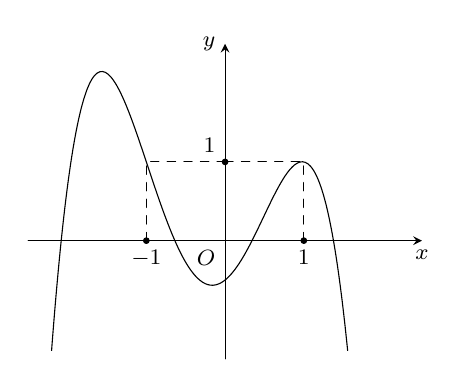
\begin{tikzpicture}[scale=1,>=stealth, font=\footnotesize, line join=round, line cap=round]
		\def\a{1} \def\b{-4} \def\c{3} % Hệ số
		\def\xmin{-2.5} \def\xmax{2.5}
		\def\ymin{-1.5} \def\ymax{2.5} 
		%	\draw[color=gray!50,dashed] (\xmin,\ymin) grid (\xmax,\ymax); 
		\draw[->] (\xmin,0)--(\xmax,0) node [below]{$x$};
		\draw[->] (0,\ymin)--(0,\ymax) node [left]{$y$};
		\node at (0,0) [below left]{$O$};
		\clip (\xmin+0.1,\ymin+0.1) rectangle (\xmax-0.5,\ymax-0.1);
		\draw[smooth,samples=300] plot(\x,{-0.8*(\x)^4+-0.8*(\x)^3+2.3*(\x)^2+0.8*(\x)-0.5});
		\draw[dashed](-1,0)|-(0,1)
		(1,0)|-(0,1);
		\draw[fill=black](-1,0)node[below]{$-1$}circle(1pt) (1,0)node[below]{$1$}circle(1pt) (0,1)node[above left]{$1$}circle(1pt);
		\end{tikzpicture}}
	\loigiai{
		\immini{
			Ta có $ f(x)-1=0\Leftrightarrow f(x)=1$.\\
			Vẽ đường thẳng $ y=1$ cắt đồ thị $ y=f(x)$ tại $3$ điểm.\\
			Suy ra phương trình $ f(x)-1=0$ có ba nghiệm thực phân biệt.}{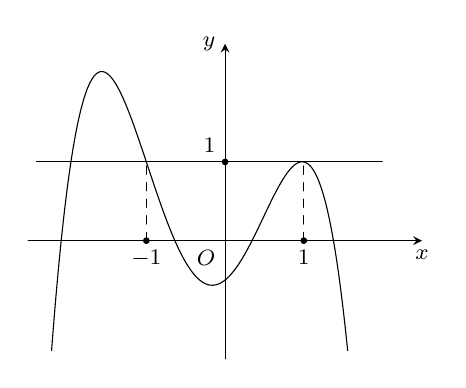
\begin{tikzpicture}[scale=1,>=stealth, font=\footnotesize, line join=round, line cap=round]
			\def\a{1} \def\b{-4} \def\c{3} % Hệ số
			\def\xmin{-2.5} \def\xmax{2.5}
			\def\ymin{-1.5} \def\ymax{2.5} 
			%	\draw[color=gray!50,dashed] (\xmin,\ymin) grid (\xmax,\ymax); 
			\draw[->] (\xmin,0)--(\xmax,0) node [below]{$x$};
			\draw[->] (0,\ymin)--(0,\ymax) node [left]{$y$};
			\node at (0,0) [below left]{$O$};
			\clip (\xmin+0.1,\ymin+0.1) rectangle (\xmax-0.5,\ymax-0.1);
			\draw[smooth,samples=300] plot(\x,{-0.8*(\x)^4+-0.8*(\x)^3+2.3*(\x)^2+0.8*(\x)-0.5});
			\draw[dashed](-1,0)|-(0,1)
			(1,0)|-(0,1);
			\draw[fill=black](-1,0)node[below]{$-1$}circle(1pt) (1,0)node[below]{$1$}circle(1pt) (0,1)node[above left]{$1$}circle(1pt);
			\draw(\xmin,1)--(\xmax,1)node[above]{$y=1$};
			\end{tikzpicture}}
	}
\end{ex}

\begin{ex}%Câu 3%[Dự án 16 - TeamTeXHoa - TT-ChuyenDH-Vinh-L1-NH21-22 - DuongPham]%[2D1Y3-1]
	\immini{	Cho hàm số $ y=f(x)$ có đồ thị như hình vẽ. Giá trị nhỏ nhất của hàm số đã cho trên $\left[0;3\right]$ bằng
		\choice
		{$ 0$}
		{\True $-1$}
		{$ 1$}
		{$ 3$}}{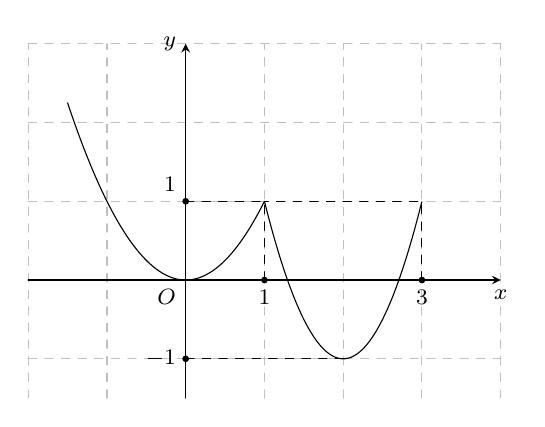
\begin{tikzpicture}[scale=1,>=stealth, font=\footnotesize, line join=round, line cap=round]
		\def\a{1} \def\b{0} \def\c{0} % Hệ số
		\def\xmin{-2} \def\xmax{4}
		\def\ymin{-1.5} \def\ymax{3}
		
		\draw[color=gray!50,dashed] (\xmin,\ymin) grid (\xmax,\ymax);
		
		\draw[->] (\xmin,0)--(\xmax,0) node [below]{$x$};
		\draw[->] (0,\ymin)--(0,\ymax) node [left]{$y$};
		\node at (0,0) [below left]{$O$};
		\clip (\xmin+0.1,\ymin+0.1) rectangle (\xmax-0.5,\ymax-0.1);
		\draw[smooth,samples=300,domain=-1.5:1] plot(\x,{\a*(\x)^2+\b*(\x)+\c});
		\draw[smooth,samples=300,domain=1:3] plot(\x,{2*(\x)^2-8*(\x)+7});
		\draw[dashed](1,0)|-(0,1) (3,0)|-(1,1); \draw[dashed](0,-1)--(2,-1);
		\draw[fill=black](3,0)node[below]{$3$}circle(1pt) (1,0)node[below]{$1$}circle(1pt) (0,1)node[above left]{$1$}circle(1pt) (0,-1)node[left]{$-1$}circle(1pt);
		\end{tikzpicture}}
	\loigiai{
		
	}
\end{ex}

\begin{ex}%Câu 4%[Dự án 16 - TeamTeXHoa - TT-ChuyenDH-Vinh-L1-NH21-22 - DuongPham]%[2D1B1-1]
	Cho hàm số $ y=f(x)$ có đạo hàm $ f'(x)=-x+1$ với mọi $ x\in\mathbb{R}$. Mệnh đề nào sau đây đúng?
	\choice
	{Hàm số đã cho nghịch biến trên $\mathbb{R}$}
	{Hàm số đã cho đồng biến trên khoảng $\left(1;+\infty\right)$}
	{\True Hàm số đã cho đồng biến trên khoảng $\left(-\infty ;1\right)$}
	{Hàm số đã cho nghịch biến trên khoảng $\left(-\infty ;1\right)$}
	\loigiai{
		Ta có $ f'(x)=-x+1>0\Leftrightarrow x<1$.\\
		Suy ra hàm số đã cho đồng biến trên khoảng $\left(-\infty ;1\right)$.
	}
\end{ex}

\begin{ex}%Câu 5%[Dự án 16 - TeamTeXHoa - TT-ChuyenDH-Vinh-L1-NH21-22 - DuongPham]%[2H2Y1-2]
	Diện tích toàn phần của hình nón có bán kính đáy bằng $2$ và độ dài đường sinh bằng $6$ là
	\choice
	{$ 8\pi $}
	{\True $ 16\pi $}
	{$ 12\pi $}
	{$ 24\pi $}
	\loigiai{
		$S_{\mathrm{tp}}=\pi rl+\pi{r^2}=\pi \cdot2\cdot6+\pi{2^2}=16\pi $.
	}
\end{ex}

\begin{ex}%Câu 6%[Dự án 16 - TeamTeXHoa - TT-ChuyenDH-Vinh-L1-NH21-22 - DuongPham]%[2D4Y2-1]
	Cho số phức $ z=1-2i$ và $w=-3+i$. Điểm biểu diễn số phức $ z-w$ là
	\choice
	{$ N\left(-2\,;\,-1\right)$}
	{$ Q\left(-3\,;\,4\right)$}
	{\True $ P\left(4\,;\,-3\right)$}
	{$ M\left(4\,;\,-1\right)$}
	\loigiai{
		$ z-w=\left(1-2i\right)-\left(-3+i\right)=4-3i$.\\
		Vậy điểm biểu diễn số phức $ z-w$ là $ P\left(4\,;\,-3\right)$.
	}
\end{ex}

\begin{ex}%Câu 7%[Dự án 16 - TeamTeXHoa - TT-ChuyenDH-Vinh-L1-NH21-22 - DuongPham]%[2H3Y3-5]
	Trong không gian $ Oxyz$, khoảng cách từ $ M\left(-1\,;\,0\,;\,3\right)$ đến mặt phẳng $(P)\colon2x-y-2z-1=0$ bằng
	\choice
	{\True 3}
	{2}
	{$\dfrac{8}{3}$}
	{$\dfrac{1}{3}$}
	\loigiai{
		$$ \mathrm{d}\left(M,(P)\right)=\dfrac{\left| 2.\left(-1\right)-0-2\cdot3-1\right|}{\sqrt{2^2+\left(-1\right)^2+\left(-2\right)^2}}=3.$$
	}
\end{ex}

\begin{ex}%Câu 8%[Dự án 16 - TeamTeXHoa - TT-ChuyenDH-Vinh-L1-NH21-22 - DuongPham]%[2D3B2-1]
	Nếu $\displaystyle\int\limits_1^2f(x)\text{d}x=3$ và $\displaystyle\int\limits_3^2f(x)\text{d}x=1$ thì $\displaystyle\int\limits_1^3f(x)\text{d}x$ bằng
	\choice
	{$ 4$}
	{$-2$}
	{\True $ 2$}
	{$-4$}
	\loigiai{
		Ta có $\displaystyle\int\limits_1^3f(x)\text{d}x=\displaystyle\int\limits_1^2f(x)\text{d}x+\displaystyle\int\limits_2^3f(x)\text{d}x=3+(-1)=2$.
	}
\end{ex}

\begin{ex}%Câu 9%[Dự án 16 - TeamTeXHoa - TT-ChuyenDH-Vinh-L1-NH21-22 - DuongPham]%[2D1B2-1]
	Cho hàm số $ y=f(x)$ có đạo hàm $f'(x)=2(x-1)^2(x-3)(x^2-4)$ với mọi $ x\in\mathbb{R}$. Số điểm cực tiểu của hàm số đã cho là
	\choice
	{\True $ 2$}
	{$ 4$}
	{$ 3$}
	{$ 1$}
	\loigiai{
		Cho $f'(x)=0\Leftrightarrow\hoac{
			& x=1\\ 
			& x=3\\ 
			& x=\pm 2.}$\\
		Bảng xét dấu:\\
		\begin{center}
			
\begin{tikzpicture}
			\tkzTabInit[nocadre=true,lgt=2,espcl=2,deltacl=0.6]
			{$x$ /0.6,$f'(x)$ /0.6}
			{$-\infty$,$-2$,$1$,$2$,$3$,$+\infty$}
			\tkzTabLine{,-,$0$,+,$0$,+,$0$,-,$0$,+,}
			\end{tikzpicture}
		\end{center}
		Dựa vào bảng xét dấu, suy ra hàm số có 2 điểm cực tiểu.
	}
\end{ex}

\begin{ex}%Câu 10%[Dự án 16 - TeamTeXHoa - TT-ChuyenDH-Vinh-L1-NH21-22 - DuongPham]%[2D2B4-2]
	Đạo hàm của hàm số $ y=\log_4(2x^2-3)$ là
	\choice
	{$y'=\dfrac{4x}{(2x^2-3)\ln 2}$}
	{$y'=\dfrac{4x}{2x^2-3}$}
	{$y'=\dfrac{1}{(2x^2-3)\ln 4}$}
	{\True $y'=\dfrac{2x}{(2x^2-3)\ln 2}$}
	\loigiai{
		Ta có $y'=\dfrac{4x}{(2x^2-3)\ln 4}=\dfrac{2x}{(2x^2-3)\ln 2}$.
	}
\end{ex}

\begin{ex}%Câu 11%[Dự án 16 - TeamTeXHoa - TT-ChuyenDH-Vinh-L1-NH21-22 - DuongPham]%[1H3K5-4]
	Cho hình chóp $S.ABCD$ có đáy $ABCD$ là hình vuông cạnh $\sqrt{3}a$, cạnh bên $ SD=\sqrt{6}a$ và $ SD$ vuông góc với mặt phẳng đáy. Khoảng cách giữa hai đường thẳng $ SB$ và $CD$ bằng
	\choice
	{$\sqrt{3}a$}
	{\True $\sqrt{2}a$}
	{$ 2a$}
	{$ a$}
	\loigiai{
		\immini{	Kẻ $ DH\perp SA$.\\
			Ta có\\ $\left.\begin{aligned}
			& AB\perp AD\\ 
			& AB\perp SD\\ 
			\end{aligned}\right\}\Rightarrow AB\perp\left(SAD\right)\Rightarrow AB\perp DH$.\\
			Lại có\\ $\left.\begin{aligned}
			& DH\perp SA\\ 
			& DH\perp AB\\ 
			\end{aligned}\right\}\Rightarrow DH\perp\left(SAB\right)\Rightarrow DH\perp SB.\quad(1)$}{
			\begin{tikzpicture}[>=stealth,line join=round,line cap=round,font=\footnotesize,scale=1]
			\def\ha{2}
			\def\aa{3}
			\def\bb{2}
			\path
			(0,0)coordinate(D)
			($(D)+(0,\ha)$)coordinate(S)
			(\aa,0)coordinate(C)
			(-135:\bb)coordinate(A)
			($(A)+(C)-(D)$)coordinate(B)
			($(S)!(D)!(A)$)coordinate(H)
			;
			\draw(S)--(A)--(B)--(C)--cycle (S)--(B);
			\draw[dashed](A)--(D)--(C) (S)--(D)--(H);
			\foreach \x/\g in {A/-90,B/-90,C/90,S/90,D/30,H/145}\fill[black](\x)circle(1pt)+(\g:.3)node{$\x$};
			\end{tikzpicture}}
		\noindent	Mặt khác, $ CD\parallel AB\Rightarrow CD\perp\left(SAD\right)\Rightarrow CD\perp DH.\quad(2)$\\
		Từ $(1)$ và $(2)\Rightarrow \mathrm{d}\left(SB,CD\right)=DH$.\\
		Xét $\triangle SAD$ vuông tại $ D$ có\\
		$\dfrac{1}{D{H^2}}=\dfrac{1}{S{D^2}}+\dfrac{1}{A{D^2}}=\dfrac{1}{6a^2}+\dfrac{1}{3a^2}=\dfrac{1}{2a^2}\Rightarrow DH=a\sqrt{2}$.
	}
\end{ex}

\begin{ex}%Câu 12%[Dự án 16 - TeamTeXHoa - TT-ChuyenDH-Vinh-L1-NH21-22 - DuongPham]%[2D2B4-3]
	Đồ thị hàm số nào sau đây \textbf{không }có đường tiệm cận ngang?
	\choice
	{\True $ y=\log_2\dfrac{1}{x}$}
	{$ y=\dfrac{1}{2^x}$}
	{$ y=\dfrac{1}{x}$}
	{$ y=\dfrac{\sqrt{1-x}}{x}$}
	\loigiai{
		Xét hàm số $ y=\log_2\dfrac{1}{x}$.\\
		Điều kiện xác định: $ x>0$.\\
		Ta có $\lim\limits_{x \to +\infty} \,y=\lim\limits_{x\to+\infty}\,\log_2\dfrac{1}{x}=-\infty $.\\
		Và	$\lim\limits_{x \to +\infty} \,\dfrac{1}{x}=0$.\\
		$\lim\limits_{x \to +\infty} \,\dfrac{1}{2^x}=0$.\\
		$\lim\limits_{x \to -\infty} \,\dfrac{\sqrt{1-x}}{x}=0$.\\
		Vậy đồ thị hàm số $ y=\log_2\dfrac{1}{x}$ không có đường tiệm cận ngang.
	}
\end{ex}
\setcounter{ex}{26}
%Câu 27
\begin{ex}%[Dự án 16 - TeamTeXHoa - TT ChuyenDH Vinh L1 - Vô Văn Tự]%[2D3B2-2]
	Nếu $\displaystyle \int f(x)\mathrm{\,d}x=F(x)+C$ thì
	\choice
	{$\displaystyle \int f(2x+3)\mathrm{\,d}x=2F(2x+3)+C$}
	{$\displaystyle \int f(2x+3)\mathrm{\,d}x=\dfrac{1}{2}F(x)+C$}
	{$\displaystyle \int f(2x+3)\mathrm{\,d}x=F(2x+3)+C$}
	{\True $\displaystyle \int f(2x+3)\mathrm{\,d}x=\dfrac{1}{2}F(2x+3)+C$}
	\loigiai{
		Đặt $t=2x+3\Rightarrow \mathrm{\,d}t=2\mathrm{\,d}x$.\\
		Ta có $\displaystyle \int f(2x+3)\mathrm{\,d}x=\displaystyle \int f(t)\cdot\dfrac{\mathrm{\,d}t}{2}=\dfrac{1}{2}\displaystyle \int f(t)\mathrm{\,d}t=\dfrac{1}{2}F(t)+C=\dfrac{1}{2}F(2x+3)+C$.
	}
\end{ex}
%Câu 28
\begin{ex}%[Dự án 16 - TeamTeXHoa - TT ChuyenDH Vinh L1 - Vô Văn Tự]%[1H3B2-3]
	Cho hình lăng trụ tam giác đều $ABC.A'B'C'$ có $AB=a$, $AA'=\sqrt{3}a$. Góc giữa hai đường thẳng $AB'$ và $CC'$ bằng
	\choice
	{\True $30^\circ$}
	{$60^\circ$}
	{$45^\circ$}
	{$90^\circ$}
	\loigiai{
		\immini{Ta có $\left(\widehat{AB',CC'}\right)=\left(\widehat{AB',AA'}\right)=\widehat{A'AB'}$.\\
			$\tan \widehat{A'AB'}=\dfrac{A'B'}{AA'}=\dfrac{1}{\sqrt{3}}\Rightarrow \widehat{A'AB'}=30^\circ$.}{\begin{tikzpicture}[scale=1, font=\footnotesize, line join=round, line cap=round, >=stealth]
			\path
			(0,0) coordinate (A)
			(2,-1.5) coordinate (B)
			(5,0) coordinate (C)
			(0,-3) coordinate (A')
			($(A')+(B)-(A)$) coordinate (B')
			($(B')+(C)-(B)$) coordinate (C')
			;
			\draw 
			(A)--(B)--(C)--cycle 
			(A)--(A')--(B')--(B)
			(B')--(C')--(C)
			(A)--(B')
			;
			\draw[dashed] 
			(A')--(C')
			;
			\foreach \p/\g in {A/170, B/-30, C/10, A'/180, B'/-45, C'/0}
			\draw[fill=black] (\p) circle (1pt) node[shift=(\g:3mm)] {$\p$};
			\end{tikzpicture}}
	}
\end{ex}
%Câu 29
\begin{ex}%[Dự án 16 - TeamTeXHoa - TT ChuyenDH Vinh L1 - Vô Văn Tự]%[2H3B3-6]
	Trong không gian $Oxyz$, cho mặt phẳng $(P)\colon x-y+2z-3=0$ và đường thẳng \\ $d\colon \dfrac{x}{-2}=\dfrac{y+1}{2}=\dfrac{z-3}{m}$. Giá trị của $m$ để $d$ vuông góc với $(P)$ là
	\choice
	{$2$}
	{\True $-4$}
	{$0$}
	{$1$}
	\loigiai{
		Ta có véc-tơ pháp tuyến mặt phẳng $(P)$ là $\overrightarrow{n}_{(P)}=(1;-1;2)$, véc-tơ chỉ phương đường thẳng $d$ là $\overrightarrow{u}_d=(-2;2;m)$. Để $d$ vuông góc với $(P)$ thì $\overrightarrow{n}_{(P)}$, $\overrightarrow{u}_d$ cùng phương, do đó $\dfrac{1}{-2}=\dfrac{-1}{2}=\dfrac{2}{m}\Rightarrow m=-4$.
	}
\end{ex}
%Câu 30
\begin{ex}%[Dự án 16 - TeamTeXHoa - TT ChuyenDH Vinh L1 - Vô Văn Tự]%[2H3B3-6]
	Với mọi số thực dương $a$, $b$ thỏa mãn $\log_2a+\log_4b=1$, khẳng định nào sau đây đúng?
	\choice
	{$a^2b=1$}
	{$ab^2=4$}
	{$ab^2=1$}
	{\True $a^2b=4$}
	\loigiai{
		Ta có $\log_2a+\log_4b=1\Leftrightarrow \log_2a+\dfrac{1}{2}\log_2b=1\Leftrightarrow \log_2a^2b=2 \Leftrightarrow a^2b=4$.
	}
\end{ex}
%Câu 31
\begin{ex}%[Dự án 16 - TeamTeXHoa - TT ChuyenDH Vinh L1 - Vô Văn Tự]%[2H2B1-2]
	Cho khối nón có góc ở đỉnh bằng $120^\circ$ và có thể tích bằng $\pi a^3$. Diện tích xung quanh của khối nón đã cho bằng
	\choice
	{\True $2\textsf{3}\pi a^2$}
	{$\sqrt{3}\pi a^2$}
	{$\pi a^2$}
	{$4\sqrt{3}\pi a^2$}
	\loigiai{
		Gọi $h$ là chiều cao khối nón, $R$ là bán kính đáy, ta có
		\[\left\{\begin{aligned}
		&\dfrac{1}{3}\pi R^2h=\pi a^3\\&\tan 60^\circ=\dfrac{R}{h}
		\end{aligned}\right. \Leftrightarrow \left\{\begin{aligned}
		&R=h\sqrt{3}\\&\pi h^3=\pi a^3
		\end{aligned}\right. \Leftrightarrow \left\{\begin{aligned}
		&R=a\sqrt{3}\\&h=a.\end{aligned}\right.\]
		Độ dài đường sinh của khối nón là $\ell =\sqrt{R^2+h^2}=2a$.\\
		Diện tích xung quanh của khối nón đã cho là $S_{\mathrm{xq}}=\pi R\ell =\pi\cdot a\sqrt{3}\cdot2a=2\sqrt{3}\pi a^2$.
	}
\end{ex}
%Câu 32
\begin{ex}%[Dự án 16 - TeamTeXHoa - TT ChuyenDH Vinh L1 - Vô Văn Tự]%[2H3B3-3]
	Trong không gian $Oxyz$, cho đường thẳng $d\colon \dfrac{x-3}{1}=\dfrac{y-2}{-1}=\dfrac{z+2}{2}$ và hai điểm $A(5;3-1)$, $B(3;1;-2)$. Tọa độ điểm $C$ thuộc $d$ sao cho tam giác $ABC$ vuông tại $B$ là
	\choice
	{$(4;1;0)$}
	{$(3;2;-2)$}
	{\True $(2;3;-4)$}
	{$(5;0;2)$}
	\loigiai{
		Tọa độ điểm $C$ có dạng $C(3+t;2-t;-2+2t)$, $\overrightarrow{BA}=(2;2;1)$, $\overrightarrow{BC}=(t;1-t;2t)$.\\
		Tam giác $ABC$ vuông tại $B\Leftrightarrow \overrightarrow{BA}\cdot \overrightarrow{BC}=0\Leftrightarrow 2t+2-2t+2t=0\Leftrightarrow t=-1$.\\
		Vậy tọa độ điểm $C$ là $(2;3;-4)$.
	}
\end{ex}
%Câu 33
\begin{ex}%[Dự án 16 - TeamTeXHoa - TT ChuyenDH Vinh L1 - Vô Văn Tự]%[2H1B3-2]
	Cho khối chóp $S.ABC$ có đáy $ABC$ là tam giác đều cạnh $2a$, mặt bên $SBC$ là tam giác vuông cân tại $S$ và $(SBC)$ vuông góc với $(ABC)$. Thể tích khối chóp đã cho bằng
	\choice
	{$3\sqrt{3}a^3$}
	{\True $\dfrac{\sqrt{3}}{3}a^3$}
	{$\dfrac{\sqrt{3}}{12}a^3$}
	{$\sqrt{3}a^3$}
	\loigiai{
		\immini{Gọi $H$ là trung điểm $BC$.\\
			Ta có $\left\{\begin{aligned}
			&(SBC)\perp (ABC)\\&(SBC)\cap (ABC)=BC\\&SH\perp BC
			\end{aligned}\right. \Rightarrow SH\perp (ABC)$.\\
			Lại có $SH=\dfrac{BC}{2}=a$, tam giác $ABC$ đều cạnh $2a$ có\\ $S=\dfrac{(2a)^2\sqrt{3}}{4}=a^2\sqrt{3}$.\\
			Do đó thể tích cần tìm là $V=\dfrac{1}{3}a\cdot a^2\sqrt{3}=\dfrac{\sqrt{3}}{3}a^3$.}{\begin{tikzpicture}[scale=1, font=\footnotesize, line join=round, line cap=round, >=stealth]
			\path
			(0,0) coordinate (B)
			(5,0) coordinate (A)
			(2,-2) coordinate (C)
			(1,3) coordinate (S)
			($(B)!0.5!(C)$) coordinate (H)
			;
			\draw 
			(S)--(B)--(C)--(A)--(S)--(H) 
			(S)--(C)
			;
			\draw[dashed] 
			(B)--(A)
			;
			\foreach \p/\g in {A/0, B/180, C/-90, S/90, H/-90}
			\draw[fill=black] (\p) circle (1pt) node[shift=(\g:3mm)] {$\p$};
			\end{tikzpicture}}
	}
\end{ex}
%Câu 34
\begin{ex}%[Dự án 16 - TeamTeXHoa - TT ChuyenDH Vinh L1 - Vô Văn Tự]%[2D4B4-1]
	Gọi $z_0$ là nghiệm phức có phần ảo âm của phương trình $z^2-8z+25=0$. Số phức liên hợp của $z_1=2-z_0$ là
	\choice
	{\True $-2-3i$}
	{$2+3i$}
	{$4-3i$}
	{$-2+3i$}
	\loigiai{
		Ta có $z^2-8z+25=0\Leftrightarrow \left[\begin{aligned}
		&z=4+3i\\&z=4-3i.\end{aligned}\right.$\\
		Suy ra $z_0=4-3i$.\\
		Do đó $z_1=2-z_0=2-(4-3i)=-2+3i\Rightarrow \overline{z}_1=-2-3i$.
	}
\end{ex}
%Câu 35
\begin{ex}%[Dự án 16 - TeamTeXHoa - TT ChuyenDH Vinh L1 - Vô Văn Tự]%[2D3K3-1]
	\immini{Cho hàm số $f(x)$ liên tục trên $\mathbb{R}$ và có đồ thị như hình vẽ bên. Biết rằng các diện tích $S_1$, $S_2$ thỏa mãn $S_1=2S_2=3$. Tích phân $\displaystyle \int\limits_0^4 f(x)\mathrm{\,d}x$ bằng
		\choice
		{$3$}
		{$\dfrac{3}{2}$}
		{\True $-\dfrac{3}{2}$}
		{$\dfrac{9}{2}$}}{\begin{tikzpicture}[scale=1,>=stealth, font=\footnotesize, line join=round, line cap=round]
		\draw[->] (-1,0)--(0,0) node[below left]{$O$}--(5,0) node[below]{$x$};
		\draw[->] (0,-2)--(0,3) node[right]{$y$};
		
		\fill[pattern=north east lines] plot[smooth,samples=100,domain=0:4] (\x,{-0.3*(\x)*(\x-2.5)*(\x-4)})--plot[smooth,samples=100,domain=4:0] (\x,{0*(\x)});
		
		\draw[domain=-0.5:4.5, samples=100] plot(\x,{-0.3*(\x)*(\x-2.5)*(\x-4)});
		\draw(4,0)node[below]{$4$};
		\draw(3.3,0)node[above]{$S_2$};
		\draw(1,-0.3)node[below]{$S_1$};
		\end{tikzpicture}}
	\loigiai{
		\immini{Ta có $f(x)=0\Leftrightarrow \left[\begin{aligned}&x=0\\&x=a~(0<a<4)\\&x=4.\end{aligned}\right.$\\
			Suy ra
			\allowdisplaybreaks
			\begin{eqnarray*}
				\displaystyle \int\limits_0^4 f(x)\mathrm{\,d}x=\displaystyle \int\limits_0^a f(x)\mathrm{\,d}x+\displaystyle \int\limits_a^4 f(x)\mathrm{\,d}x &=& -S_1+S_2 \\ &=& -3+\dfrac{3}{2}=-\dfrac{3}{2}.
		\end{eqnarray*} }{\begin{tikzpicture}[scale=1,>=stealth, font=\footnotesize, line join=round, line cap=round]
			\draw[->] (-1,0)--(0,0) node[below left]{$O$}--(5,0) node[below]{$x$};
			\draw[->] (0,-2)--(0,3) node[right]{$y$};
			\draw[domain=-0.5:4.5, samples=100] plot(\x,{-0.3*(\x)*(\x-2.5)*(\x-4)});
			\draw(2.5,0)node[below]{$a$};
			\draw(4,0)node[below]{$4$};
			\draw(3.3,0)node[above]{$S_2$};
			\draw(1,-0.3)node[below]{$S_1$};
			\end{tikzpicture}}
	}
\end{ex}
%Câu 36
\begin{ex}%[Dự án 16 - TeamTeXHoa - TT ChuyenDH Vinh L1 - Vô Văn Tự]%[2D1K1-2]
	\immini{Cho hàm số bậc ba $y=f(x)$. Đồ thị hàm số $f'(x)$ như hình vẽ bên. Hàm số $g(x)=f(x)+\dfrac{1}{x}$ nghịch biến trên khoảng nào sau đây?
		\choice
		{$(2;+\infty)$}
		{$(-1;2)$}
		{\True $(0;2)$}
		{$(-\infty;-1)$}}{\begin{tikzpicture}[scale=1,>=stealth, font=\footnotesize, line join=round, line cap=round]
		\draw[->] (-2,0)--(3,0) node[below]{$x$};
		\draw[->] (0,-2)--(0,2.5) node[right]{$y$};
		\draw[domain=-1.6:2.6, samples=100] plot(\x,{0.5*(\x+1)*(\x-2)});
		\draw(-1,0)node[below left]{$-1$} circle(1pt);
		\draw(2,0)node[below]{$2$} circle(1pt) (0,0) node[below right]{$O$} circle(1pt);
		\end{tikzpicture}}
	\loigiai{
		\immini{Ta có $g'(x)=f'(x)-\dfrac{1}{x^2}$.\\
			Hàm số $g(x)$ nghịch biến $\begin{aligned}[t]
			&\Leftrightarrow g'(x)\le 0 \\
			&\Leftrightarrow f'(x)-\dfrac{1}{x^2}\le0\\
			&\Leftrightarrow f'(x)\le \dfrac{1}{x^2}.
			\end{aligned}$\\
			Khi đó đồ thị $f'(x)$ phải nằm phía dưới đồ thị hàm số $\dfrac{1}{x^2}$.\\
			Dựa vào đồ thị và kết hợp điều kiện $x\ne0$ ta chọn đáp án là $(0;2)$.}{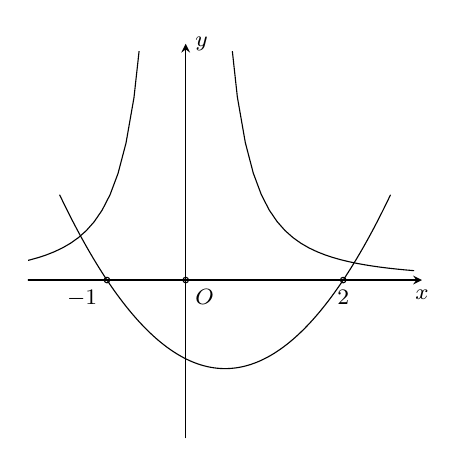
\begin{tikzpicture}[scale=1,>=stealth, font=\footnotesize, line join=round, line cap=round]
			\draw[->] (-2,0)--(3,0) node[below]{$x$};
			\draw[->] (0,-2)--(0,3) node[right]{$y$};
			\draw[domain=-1.6:2.6, samples=100] plot(\x,{0.5*(\x+1)*(\x-2)});
			\clip (-2,-2) rectangle (2.9,2.9);
			\draw[samples=100] plot(\x,{1/((\x)^2)});
			\draw
			(-1,0)node[below left]{$-1$} circle(1pt)
			(2,0)node[below]{$2$} circle(1pt) 
			(0,0) node[below right]{$O$} circle(1pt);
			\end{tikzpicture}}
	}
\end{ex}



%---Câu 37
\begin{ex}%[1D2K5-2]
	An và Bình cùng chơi một trò chơi, mỗi lượt chơi một bạn đặt úp năm tấm thẻ, trong đó có hai thẻ ghi số $2$, hai thẻ ghi số $3$ và một thẻ ghi số $4$, bạn còn lại chọn ngẫu nhiên ba thẻ trong năm tấm thẻ đó. Người chọn thẻ thắng lượt chơi nếu tổng các số trên ba tấm thẻ được chọn bằng $8$, ngược lại người kia sẽ thắng. Xác suất để An thắng lượt chơi khi An là người chọn thẻ bằng
	\choice
	{$\dfrac{1}{5}$}
	{$\dfrac{1}{10}$}
	{$\dfrac{3}{20}$}
	{\True $\dfrac{3}{10}$}
	\loigiai{
		Số trường hợp xảy ra khi chọn $3$ thẻ trong $5$ tấm thẻ là $n\left( \Omega \right)=\mathrm{C}_5^3=10$.\\
		Gọi $A$ là biến cố để An thắng lượt chơi.\\
		Số các trường hợp xảy ra cho $A$ là
		\begin{itemize}
			\item  $2$ thẻ số $2$ và một thẻ số $4$ có $1$ cách.
			\item  $2$ thẻ số $3$ và $1$ thẻ số $2$ có $2$ cách.
		\end{itemize}
		Suy ra số các trường hợp xảy ra cho A là $n\left( A \right)=3$.\\
		Vậy $\mathrm{P}\left( A \right)=\dfrac{n\left( A \right)}{n\left( \Omega \right)}=\dfrac{3}{10}$.
	}
\end{ex}

\begin{ex}%[2D2K4-4]
	Gọi $m$ là giá trị nhỏ nhất của hàm số $f\left( x \right)=4^x+\left( a-2 \right)2^x+2$ trên đoạn $\left[-1;1 \right]$. Tất cả giá trị của $a$ để $m\ge 1$ là
	\choice
	{$a\ge 1$}
	{$-\dfrac{1}{2}\le a\le 0$}
	{$a\le -\dfrac{1}{2}$}
	{\True $a\ge 0$}
	\loigiai{
		Đặt $t=2^x,t\in \left[\dfrac{1}{2};2 \right]$, $f\left( x \right)$ trở thành $g\left( t \right)=t^2+\left( a-2 \right)t+2$.\\
		Hàm số $g\left( t \right)$ liên tục trên $\left[\dfrac{1}{2};2 \right]$.\\
		Ta có $g'\left( t \right)=2t+a-2$.\\
		Cho $g'\left( t \right)=0\Leftrightarrow t=\dfrac{2-a}{2}$.
		\begin{description}
			\item[Trường hợp 1:] $\dfrac{1}{2}\le \dfrac{2-a}{2}\le 2\Leftrightarrow -2\le a\le 1$.\\
			Suy ra $\underset{\left[\tfrac{1}{2};2 \right]}{\mathop{\min g\left( t \right)}}=g\left( \dfrac{2-a}{2} \right)=\dfrac{8-\left( a-2 \right)^2}{4}$.\\
			Yêu cầu bài toán $\Leftrightarrow \dfrac{8-\left( a-2 \right)^2}{4}\ge 1\Leftrightarrow 0\le a\le 4$.\\
			Vậy $0\le a\le 1$.
			\item[Trường hợp 2:] $\dfrac{2-a}{2}<\dfrac{1}{2}\Leftrightarrow a>1$.\\
			Suy ra $\underset{\left[\tfrac{1}{2};2 \right]}{\mathop{\min g\left( t \right)}}=g\left( \dfrac{1}{2} \right)=\dfrac{1}{2}a+\dfrac{5}{4}$.\\
			Yêu cầu bài toán $\Leftrightarrow \dfrac{1}{2}a+\dfrac{5}{4}\ge 1\Leftrightarrow a\ge -\dfrac{1}{2}$.\\
			Vậy $a>1$.
			\item[Trường hợp 3:] $\dfrac{2-a}{2}>2\Leftrightarrow a<-2$.\\
			Suy ra $\underset{\left[\tfrac{1}{2};2 \right]}{\mathop{\min g\left( t \right)}}=g\left( 2 \right)=2a+2$.\\
			Yêu cầu bài toán $\Leftrightarrow 2a+2\ge 1\Leftrightarrow a\ge -\dfrac{1}{2}$.\\
			Vậy không tồn tại $a$.
		\end{description}
		Kết hợp $3$ trường hợp, ta có $a\ge 0$.
	}
\end{ex}

\begin{ex}%[2D4K4-2]
	Biết phương trình $z^2+mz+m^2-2=0$ ($m$ là tham số thực) có hai nghiệm phức $z_1$, $z_2$. Gọi $A$,$B$,$C$ lần lượt là điểm biểu diễn các số phức $z_1$, $z_2$ và $z_0=i$. Có bao nhiêu giá trị của tham số $m$ để diện tích tam giác $ABC$ bằng $1$?
	\choice
	{$2$}
	{$3$}
	{\True $4$}
	{$6$}
	\loigiai{
		Ta có $\Delta =m^2-4\left( m^2-2 \right)=-3m^2+8$.
		\begin{description}
			\item[Trường hợp 1:] $\Delta >0\Leftrightarrow -3m^2+8>0\Leftrightarrow \dfrac{-2\sqrt{6}}{3}<m<\dfrac{2\sqrt{6}}{3}$.\\ 
			Khi đó, phương trình có hai nghiệm thực phân biệt là $z_1,z_2$.\\
			Vì $A,B\in Ox$ nên $AB=\left| z_1-z_2 \right|=\sqrt{\left( z_1-z_2 \right)^2}=\sqrt{\left( z_1+z_2 \right)^2-4z_1z_2}=\sqrt{-3m^2+8}$.\\
			Mặt khác, ta có $C\left( 0;1 \right)\Rightarrow \mathrm{d}\,\left( C;AB \right)=1$.\\
			$\Rightarrow {S_{\triangle ABC}}=\dfrac{1}{2}AB\cdot  \mathrm{d}\,\left( C;AB \right)=\dfrac{\sqrt{-3m^2+8}}{2}=1\Leftrightarrow m=\pm \dfrac{2\sqrt{3}}{3}$.
			\item[Trường hợp 2:] $\Delta <0\Leftrightarrow -3m^2+8<0\Leftrightarrow \hoac{& m>\dfrac{2\sqrt{6}}{3} \\&
				m<\dfrac{-2\sqrt{6}}{3}.}$\\ 
			Khi đó, phương trình có hai nghiệm phức liên hợp là $z_{1,2}=\dfrac{-m+i\sqrt{\left| \Delta \right|}}{2}$.\\
			Ta có $AB=\left| z_1-z_2 \right|=\left| i\sqrt{\left| \Delta \right|} \right|=\sqrt{\left| -3m^2+8 \right|}=\sqrt{3m^2-8}$ và $C\left( 0;1 \right)$.\\
			Phương trình đường thẳng $AB$ là $x+\dfrac{m}{2}=0$ nên $ \mathrm{d}\,\left( C;AB \right)=\dfrac{\left| m \right|}{2}$.\\
			$\Rightarrow S_{\triangle ABC}=\dfrac{1}{2}AB\cdot  \mathrm{d}\,\left( C;AB \right)=\dfrac{\left| m \right|\sqrt{3m^2-8}}{4}=1\Leftrightarrow \hoac{&m^2=4 \\&m^2=-\dfrac{4}{3}}
			\Leftrightarrow m^2=4 \Leftrightarrow m=\pm 2$.\\
		\end{description}
		Vậy có $4$ giá trị thực của tham số $m$ thỏa mãn đề bài.
	}
\end{ex}

\begin{ex}%[2D3G3-1]
	Cho hàm số $y=x^4+bx^3+cx^2+dx+e\left( b,c,d,e\in \mathbb{R} \right)$ có các giá trị cực trị là $1$,$4$ và $9$. Diện tích hình phẳng giới hạn bởi đồ thị hàm số $g\left( x \right)=\dfrac{f'\left( x \right)}{\sqrt{f\left( x \right)}}$ với trục hoành bằng
	\choice
	{$4$}
	{\True $6$}
	{$2$}
	{$8$}
	\loigiai{
		Gọi $m,n,p\left( m<n<p \right)$ lần lượt là các điểm cực trị của hàm số $y=f\left( x \right)$.\\
		Ta có bảng xét dấu của $f'\left( x \right)$ như sau
		\begin{center}
			
\begin{tikzpicture}
			\tkzTabInit[nocadre,lgt=2,espcl=2,deltacl=0.5]{$x$/1 ,$f'(x)$/1}
			{$-\infty$ , $m$ , $n$ , $p$ ,$+\infty$}
			\tkzTabLine{ , - , 0 , + , 0 , - , 0 , + , }
			\end{tikzpicture}
		\end{center}
		Khi đó hàm số đạt cực tiểu $m,p$ và đạt cực đại tại $x=n\Rightarrow f\left( n \right)=9$.\\
		Diện tích hình phẳng giới hạn bởi đồ thị hàm số $g\left( x \right)=\dfrac{f'\left( x \right)}{\sqrt{f\left( x \right)}}$ với trục hoành là
		\allowdisplaybreaks
		\begin{eqnarray*}
			S
			&=&\int\limits_m^p\left| g\left( x \right) \right|\mathrm{\,d}x
			=\left| \int\limits_m^ng\left( x \right)\mathrm{\,d}x \right|+\left| \int\limits_n^pg\left( x \right)\mathrm{\,d}x \right|
			= \int\limits_m^ng\left( x \right)\mathrm{\,d}x-\int\limits_n^pg\left( x \right)\mathrm{\,d}x\\
			&=&2\left. \left[\sqrt{f\left( x \right)} \right] \right|_m^n-2\left. \left[\sqrt{f\left( x \right)} \right] \right|_n^p=2\left[\sqrt{f\left( n \right)}-\sqrt{f\left( m \right)} \right]-2\left[\sqrt{f\left( p \right)}-\sqrt{f\left( n \right)} \right]\\
			&=& 4\sqrt{f\left( n \right)}-2\left( \sqrt{f\left( m \right)}+\sqrt{f\left( p \right)} \right)=4\cdot 3-2\cdot \left( 1+2 \right)=6.
		\end{eqnarray*} 
	}
\end{ex}

\begin{ex}%[2D1G2-2]
	\immini{
		Cho hàm số bậc ba $y=f\left( x \right)$. Biết rằng hàm số $y=f'\left( 1-x^2 \right)$ có đồ thị như hình vẽ. Số điểm cực trị của hàm số $g\left( x \right)=f\left( \dfrac{x^2-1}{x^2} \right)+\dfrac{2}{x}$ là
		\choice
		{\True $5$}
		{$4$}
		{$3$}
		{$7$}
	}{
		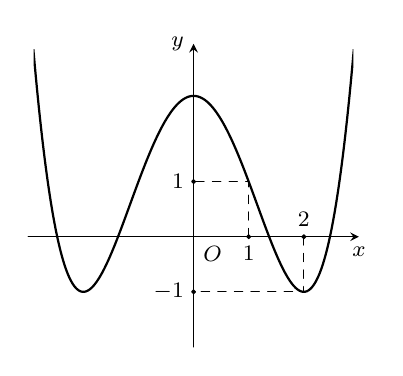
\begin{tikzpicture}[scale=0.7,>=stealth, font=\footnotesize, line join=round, line cap=round]
		\def\a{2/9} \def\b{-16/9} \def\c{23/9}
		\def\xmin{-3} \def\xmax{3}
		\def\ymin{-2} \def\ymax{3.5} 
		%	\draw[color=gray!50,dashed] (\xmin,\ymin) grid (\xmax,\ymax); 
		\draw[->] (\xmin,0)--(\xmax,0) node [below]{$x$};
		\draw[->] (0,\ymin)--(0,\ymax) node [left]{$y$};
		\node at (0,0) [below right]{$O$};
		\clip (\xmin+0.1,\ymin+0.1) rectangle (\xmax-0.1,\ymax-0.1);
		\draw[smooth,samples=300,thick] plot(\x,{\a*(\x)^4+\b*(\x)^2+\c});
		\draw[dashed](1,0)|-(0,1)  (2,0)|-(0,-1);
		\draw[fill=black]
		(2,0)node[above]{$2$}circle(1pt)
		(1,0)node[below]{$1$}circle(1pt)
		(0,-1)node[left]{$-1$}circle(1pt)
		(0,1)node[left]{$1$}circle(1pt);
		\end{tikzpicture}
	}
	\loigiai{
		Ta có $g'\left( x \right)=\dfrac{2}{x^3}\cdot f'\left( \dfrac{x^2-1}{x^2} \right)-\dfrac{2}{x^2}=\dfrac{2}{x^2}\left[\dfrac{1}{x}\cdot f'\left( \dfrac{x^2-1}{x^2} \right)-1 \right]$.\\
		$\Rightarrow g'\left( x \right)=0
		\Leftrightarrow \dfrac{1}{x}\cdot f'\left( \dfrac{x^2-1}{x^2} \right)-1=0
		\Rightarrow f'\left( \dfrac{x^2-1}{x^2} \right)=x
		\Leftrightarrow f'\left( 1-\dfrac{1}{x^2} \right)=x$.
		\immini{
			Đặt $t=\dfrac{1}{x}\Rightarrow x=\dfrac{1}{t}$ ta được $f'\left( 1-t^2 \right)=\dfrac{1}{t}$.\\
			Xét hàm số $h\left( t \right)=\dfrac{1}{t}\left( t\ne 0 \right)\Rightarrow h'\left( t \right)=-\dfrac{1}{t^2}<0,\forall t\ne 0$.\\
			Vẽ đồ thị hàm $h\left( t \right)=\dfrac{1}{t}$ trên cùng hệ trục toạ độ với hàm số $y=f'\left( 1-t^2 \right)$.\\
			Từ đồ thị suy ra $g'\left( x \right)=0$ có $5$ nghiệm đơn.\\
			Vậy hàm số $g\left( x \right)=f\left( \dfrac{x^2-1}{x^2} \right)+\dfrac{2}{x}$ có $5$ điểm cực trị.
		}{
			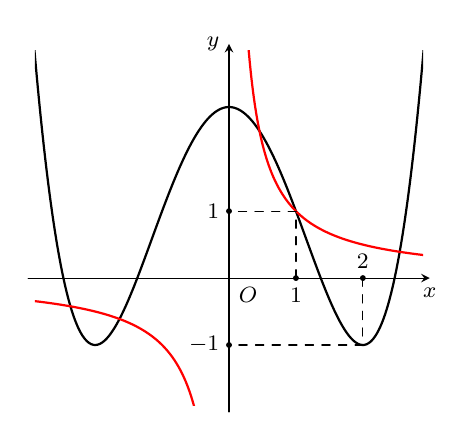
\begin{tikzpicture}[scale=0.85,>=stealth, font=\footnotesize, line join=round, line cap=round]
			\def\a{2/9} \def\b{-16/9} \def\c{23/9}
			\def\xmin{-3} \def\xmax{3}
			\def\ymin{-2} \def\ymax{3.5} 
			%	\draw[color=gray!50,dashed] (\xmin,\ymin) grid (\xmax,\ymax); 
			\draw[->] (\xmin,0)--(\xmax,0) node [below]{$x$};
			\draw[->] (0,\ymin)--(0,\ymax) node [left]{$y$};
			\node at (0,0) [below right]{$O$};
			\clip (\xmin+0.1,\ymin+0.1) rectangle (\xmax-0.1,\ymax-0.1);
			\draw[smooth,samples=300,thick] plot(\x,{\a*(\x)^4+\b*(\x)^2+\c});
			\draw[red,smooth,samples=300,thick,domain=0.1:\xmax] plot(\x,{1/(\x)});
			\draw[red,smooth,samples=300,thick,domain=\xmin:-0.1] plot(\x,{1/(\x)});
			\draw[dashed](1,0)|-(0,1)  (2,0)|-(0,-1);
			\draw[fill=black]
			(2,0)node[above]{$2$}circle(1pt)
			(1,0)node[below]{$1$}circle(1pt)
			(0,-1)node[left]{$-1$}circle(1pt)
			(0,1)node[left]{$1$}circle(1pt);
			\end{tikzpicture}
		}
	}
\end{ex}





\begin{ex}%[2H1K3-2] 
	Cho khối hộp $ABCD.A'B'C'D'$ có đáy $ABCD$ là hình thoi cạnh $a$, $\widehat{ABC}=120^\circ $. Hình chiếu vuông góc của $D'$ lên $\left( ABCD \right)$ trùng với giao điểm của $AC$ và $BD$, góc giữa hai mặt phẳng $\left( ADD'A' \right)$ và $\left( A'B'C'D' \right)$ bằng $45^\circ $. Thể tích khối hộp đã cho bằng
	\choice
	{\True $\dfrac{3}{8}a^3$}
	{$\dfrac{1}{8}a^3$}
	{$\dfrac{3}{16}a^3$}
	{$\dfrac{3}{4}a^3$}
	\loigiai{
		\immini{
			Gọi $O$ là giao của $AC$ và $BD$. Ta có $D'O\perp \left( ABCD \right)$.\\
			Mà $ABCD$ là hình thoi cạnh $a$, $\widehat{ABC}=120^\circ $ nên tam giác $ABD$ đều cạnh $a$.\\
			Gọi $H$ là trung điểm của $AD$ và $K$ là trung điểm của $HD$ suy ra $BH\perp AD$ và $BH=\dfrac{a\sqrt{3}}{2}$.\\
			Suy ra $OK\parallel BH$ và $OK=\dfrac{1}{2}BH=\dfrac{a\sqrt{3}}{4}$.\\
			Từ đó, suy ra $OK\perp AD$.\\
			Mà $D'O\perp \left( ABCD \right)\Rightarrow D'O\perp AD$.\\
			Nên $AD\perp \left( D'OK \right)\Rightarrow AD\perp D'K$.
		}{
			\begin{tikzpicture}[scale=1, font=\footnotesize, line join=round, line cap=round, >=stealth]
			\def\ad{4} % cạnh AD
			\def\ba{2} % cạnh BA
			\def\h{3} % đường cao
			\def\gocB{-150} % góc B của đáy
			\coordinate[label=above right:$D$] (D) at (0,0);
			\coordinate[label=below left:$A$] (A) at (\gocB:\ba);
			\coordinate[label=right:$C$] (C) at (\ad,0);
			\coordinate[label=below right:$B$] (B) at ($(A)+(C)-(D)$);
			\coordinate[label=below:$O$] (O) at ($(A)!0.5!(C)$);
			\coordinate[label=above:$D'$] (D') at ($(O)+(90:\h)$);
			\coordinate[label=above left:$A'$] (A') at ($(A)+(D')-(D)$);
			\coordinate[label=above right:$C'$] (C') at ($(C)+(D')-(D)$);
			\coordinate[label=above:$B'$] (B') at ($(A')+(C')-(D')$);
			\coordinate[label=above left:$K$] (K) at ($(D)!0.25!(A)$);
			\coordinate[label=above left:$H$] (H) at ($2*(K)-(D)$);
			\draw (A')--(B')--(C')--(D')--cycle (A)--(B)--(B') (B)--(C)--(C') (A)--(A');
			\draw[dashed] (A)--(D)--(C)--(A) (B)--(D)--(D')--(O) (B)--(H) (O)--(K)--(D');
			\foreach \diem in {A,B,C,D,A',B',C',D',K,H}\fill (\diem)circle(1.pt);
			%------Định nghĩa góc vuông
			\newcommand{\gocv}[4][black]{\draw[#1] ($(#3)!5pt!(#2)$)--($(#3)!2!($($(#3)!5pt!(#2)$)!.5!($(#3)!5pt!(#4)$)$)$)--($(#3)!5pt!(#4)$);}
			\gocv{O}{K}{D}
			\gocv{O}{H}{D}
			\gocv{D'}{O}{C}
			\gocv{D'}{O}{D}
			\end{tikzpicture}
		}
		\noindent
		Do đó góc giữa hai mặt phẳng $\left( ADD'A' \right)$ và $\left( A'B'C'D' \right)$ bằng $\widehat{D'KO}=45^\circ $ hay tam giác $D'KO$ vuông cân tại $O\Rightarrow D'O=OK=\dfrac{a\sqrt{3}}{4}$.\\
		Lại có diện tích hình thoi $ABCD$ bằng $S_{ABCD}=2S_{ABD}=2\cdot\dfrac{a^2\sqrt{3}}{4}=\dfrac{a^2\sqrt{3}}{2}$.\\
		Vậy thể tích của khối hộp là $V=D'O\cdot S_{ABCD}=\dfrac{a\sqrt{3}}{4}\cdot \dfrac{a^2\sqrt{3}}{2}=\dfrac{3}{8}a^3$.
	}
\end{ex}





\begin{ex}%[2H2K2-2]
	Cho hình chóp $S.ABC$ có mặt phẳng $\left( ABC \right)$ đồng thời vuông góc với hai mặt phẳng $\left( SAC \right)$ và $\left( SBC \right)$, $AC=2\sqrt{3}a$, $\widehat{ABC}=60^\circ $, đường thẳng $SA$ tạo với $\left( ABC \right)$ một góc $30^\circ$. Diện tích của mặt cầu ngoại tiếp hình chóp đã cho bằng
	\choice
	{$32\pi a^2$}
	{$5\pi a^2$}
	{$\dfrac{5}{3}\pi a^2$}
	{\True $20\pi a^2$}
	\loigiai{
		\immini{
			Mặt phẳng $\left( ABC \right)$ đồng thời vuông góc với hai mặt phẳng $\left( SAC \right)$ và $\left( SBC \right)\Rightarrow SC\perp \left( ABC \right)$.\\
			Đường thẳng $SA$ tạo với $\left( ABC \right)$ một góc $30^\circ \Rightarrow \widehat{SAC}=30^\circ $; $SC=2a$
			Gọi $O$ là tâm đường tròn ngoại tiếp $\Delta ABC$.\\
			Theo định lý sin trong tam giác $\Delta ABC$ ta có 
			\[2\mathrm{O}C=\dfrac{AC}{\sin \widehat{ABC}}=\dfrac{2\sqrt{3}a}{\sin 60^\circ}=4a\Rightarrow OC=2a.\]
		}{
			\begin{tikzpicture}[scale=1, font=\footnotesize, line join=round, line cap=round, >=stealth]
			\def\ac{4} % cạnh AC
			\def\ba{2} % cạnh BA
			\def\h{2.5} % đường cao
			\def\gocB{-45} % góc B của đáy
			\coordinate[label=left:$C$] (C) at (0,0);
			\coordinate[label=below:$A$] (A) at (\gocB:\ba);
			\coordinate[label=right:$B$] (B) at (\ac,0);
			\coordinate[label=above:$S$] (S) at ($(C)+(90:\h)$);
			\coordinate[label=below left:$M$] (M) at ($(C)!0.5!(A)$);
			\coordinate[label=below:$O$] (O) at ($(B)!2/3!(M)$);
			\coordinate[label=right:$I$] (I) at ($(S)!0.5!(C)+(O)-(C)$);
			\draw (S)--(A)--(C)--cycle (S) -- (B)--(A);
			\draw[dashed] (M)--(B)--(C) ($(S)!0.5!(C)$)--(I)--(O) (I)--(C);
			\foreach \diem in {A,B,C,S,M,O,I}	\fill (\diem)circle(1.pt);
			%------Định nghĩa góc vuông
			\newcommand{\gocv}[4][black]{\draw[#1] ($(#3)!5pt!(#2)$)--($(#3)!2!($($(#3)!5pt!(#2)$)!.5!($(#3)!5pt!(#4)$)$)$)--($(#3)!5pt!(#4)$);}
			\gocv{S}{C}{B}
			\gocv{S}{C}{A}
			%\foreach \x/\y/\z in {S/A/B,S/A/C,A/B/C,B/M/C} 
			%\draw pic[draw=black,angle radius=0.2cm]{right angle=\x--\y--\z};
			\end{tikzpicture}
		}
		\noindent
		Từ $O$ dựng trục $\triangle ABC$ là đường thẳng $\Delta $, $\Delta \parallel SC$.\\
		Trong mặt phẳng $\left( SC;\Delta \right)$, đường trung trực cạnh $SC$ cắt trục $\triangle ABC$ tại $I$, ta có $I$ là tâm mặt cầu ngoại tiếp hình chóp $S.ABC$.\\
		Suy ra $R=IC=\sqrt{OC^2+OI^2}=\sqrt{4a^2+a^2}=a\sqrt{5}$.\\
		Diện tích mặt cầu $S=4\pi\left( a\sqrt{5} \right)^2=20\pi a^2$.
	}
\end{ex}

\begin{ex}%[2H3K3-2] 
	Trong không gian $Oxyz$, đường thẳng vuông góc chung của hai đường thẳng\break $d_1\colon \dfrac{x-2}{2}=\dfrac{y-3}{3}=\dfrac{z+4}{-5}$ và $d_2\colon \dfrac{x+1}{3}=\dfrac{y-4}{-2}=\dfrac{z-4}{-1}$ đi qua điểm nào trong các điểm sau đây?
	\choice
	{\True $M\left( 1;1;2 \right)$}
	{$N\left( 2;2;2 \right)$}
	{$P\left( -1;1;0 \right)$}
	{$Q\left( 2;1;3 \right)$}
	\loigiai{
		Đường vuông góc chung cắt $d_1$; $d_2$ lần lượt tại $A$; $B$.\\
		Suy ra $\heva{& A\in d_1\Rightarrow A\left( 2+2t;3+3t;-4-5t \right),t\in \mathbb{R}\\&
			B\in d_2\Rightarrow B\left( -1+3m;4-2m;4-m \right),m\in \mathbb{R}.}
	\\	\Rightarrow \overrightarrow{AB}=\left( 3m-2t-3;1-2m-3t;8+5t-m \right)$.\\
		Ta có $d_1$ có véc-tơ chỉ phương $\overrightarrow{u}\left( 2;3;-5 \right)$; $d_2$ có véc-tơ chỉ phương $\overrightarrow{v}=\left( 3;-2;-1 \right)$.\\
		Ta có 
		$\heva{&\overrightarrow{AB}\cdot \overrightarrow{u}=0 \\&\overrightarrow{AB}\cdot \overrightarrow{v}=0}
		\Leftrightarrow \heva{&5m-38t=43 \\&14m-5t=19}
		\Leftrightarrow \heva{&t=-1 \\&m=1}
		\Rightarrow \heva{& \overrightarrow{AB}=\left( 2;2;2 \right)=2\left( 1;1;1 \right)\\& A\left( 0;0;1 \right).}$\\
		Phương trình đường vuông góc chung $\dfrac{x}{1}=\dfrac{y}{1}= \dfrac{z-1}{1} \Rightarrow M$ thuộc đường vuông góc chung.
	}
\end{ex}






\setcounter{ex}{44}
\begin{ex} %[2D2G6-5]% cau 45
	Số nghiệm nguyên của bất phương trình $\sqrt{2{{\log }_{2}}(x+2)}-\sqrt{{{\log }_{2}}( 2x^2-1 )}\ge ( x+1 )( x-5 )$ là
	\choice 
	{$ 5 $}
	{\True $ 6 $}
	{$ 7 $}
	{$ 4 $}
	\loigiai{
		Điều kiện $\heva{
			& x+2\ge 1 \\ 
			& 2x^2-1\ge 1 
		}\Leftrightarrow \heva{
			& x\ge -1 \\ 
			& \hoac{
				& x\le -1 \\ 
				& x\ge 1 
			} 
		}\Leftrightarrow \hoac{
			& x=-1 \\ 
			& x\ge 1.
		}$\\
		Nhận xét $x=-1$ là nghiệm của bất phương trình.
		Với $x\ge 1$ ta có:
		\allowdisplaybreaks
		\begin{eqnarray*}
			& \sqrt{2{{\log }_{2}}(x+2)}-\sqrt{{{\log }_{2}}( 2x^2-1 )}\ge ( x+1 )( x-5 ) \\ 
			& \Leftrightarrow \sqrt{{{\log }_{2}}(x^2+4x+4)}-\sqrt{{{\log }_{2}}( 2x^2-1 )}\ge x^2-4x-5. \quad ( 2 ) 
		\end{eqnarray*}\\
		Đặt $\heva{
			& a=2x^2-1 \\ 
			& b=x^2+4x+4 
		}( a\ge 1\,;\,b\ge 1 )$.\\
		$( 2 )\Leftrightarrow b+\sqrt{{{\log }_{2}}b}\ge a+\sqrt{{{\log }_{2}}a}. \quad ( 3 )$\\
		Xét hàm số $f( t )=t+\sqrt{{{\log }_{2}}t}$ với $t\ge 1$.\\
		$f'( t )=1+\dfrac{1}{2t\sqrt{{{\log }_{2}}t\,}\ln 2}>0,\,\forall t>1$.\\
		Hàm số $f( t )$ đồng biến trên khoảng $( 1\,;\,+\infty )$ nên từ $( 3 )$ ta có \\
		$b\ge a\Leftrightarrow x^2+4x+4\ge 2x^2-1\Leftrightarrow -x^2+4x+5\ge 0\Leftrightarrow -1\le x\le 5$.\\
		Mà $x\ge 1\Rightarrow 1\le x\le 5$.\\
		Vậy có 6 giá trị nguyên của $x$ thỏa mãn.
	} 
\end{ex}
%%==========
\begin{ex}%[2D4G5-1] %cau 46
	Gọi $S$ là tập hợp tất cả các số phức $z$ thỏa mãn điều kiện $z \cdot \overline{z}=\left| z+\overline{z}\right| $. 
	Xét các số phức $z_1, z_2 \in S$ sao cho $\left| {z}_{1}-{z}_{2} \right| =1$. Giá trị nhỏ nhất của biểu thức $P=\left| z_1-\sqrt{3}i \right| +\left|  \overline{{{z}_{2}}}+\sqrt{3}i \right| $ bằng
	\choice 
	{\True $2$}
	{$1+\sqrt{3}$}
	{$2\sqrt{3}$}
	{$\sqrt{20-8\sqrt{3}}$}
	\loigiai{
		Đặt $z=a+bi\; (a,b\in \mathbb{R})$.
		Ta có $z\cdot \overline{z}=\left|  z+\overline{z} \right| \Leftrightarrow a^2+b^2=2|a|\Leftrightarrow \hoac {
			& a^2+b^2=2a \\ 
			& a^2+b^2=-2a.}$\\
		Gọi $A$, $B$ lần lượt là hai điểm biểu diễn của số phức ${{z}_{1}},{{z}_{2}}$.\\
		$\left| {{z}_{1}}-{{z}_{2}} \right| =1\Rightarrow AB=1$.\\
		Khi đó $P=\left|  {{z}_{1}}-\sqrt{3}i \right| +\left|  \overline{{{z}_{2}}}+\sqrt{3}i \right| =CA+CB$, với $C(0;\sqrt{3})$.\\
		$\Rightarrow {{P}_{\min }}\ge {{I}_{1}}C-R+{{I}_{2}}C-R=2$; với ${{I}_{1}}(-1;0),{{I}_{2}}(1;0),R=1$.\\
		Dấu \lq\lq $=$ \rq\rq \, xảy ra vì $A,B$ lần lượt là trung điểm $C{{I}_{1}},C{{I}_{2}}$ và $AB=\dfrac{{{I}_{1}}{{I}_{2}}}{2}=1$ (thỏa mãn).
		\begin{center}
			\begin{tikzpicture}[>=latex,line join=round,line cap=round,line width=0.8pt,font=\footnotesize,x=1cm,y=1cm]
			\draw[->](-2.5,0)--(0,0)node [above right=-2pt]{$ O $}--(3,0) node [above]{$ x $};
			\draw[->](0,-1.5)--(0,3)node [right]{$ y $};
			\coordinate (I1) at (-1,0);
			\coordinate (I2) at (1,0);
			\coordinate[label=above right:$C$](C) at (0,1.732); % 
			\coordinate [label=above left:$A$](A) at ($ (I1)!0.5!(C) $);
			\coordinate [label=above right:$B$](B) at ($ (I2)!0.5!(C) $);
			\node [below] at (-1,0) {$ I_1 $};
			\node [below] at (1,0) {$ I_2 $};
			\fill (-1,0) circle (1.5pt) (1,0)circle (1.5pt)(C)circle (1.5pt)(A)circle (1.5pt)(B)circle (1.5pt);
			\draw (-1,0) circle[radius=1cm]; % Hoặc dùng lệnh \draw (0,0) circle (1cm);
			\draw (1,0) circle[radius=1cm];
			\draw (C)--(I1);
			\draw (C)--(I2);
			\draw (A)--(B);
			\end{tikzpicture}
		\end{center}	
	} 
\end{ex}
\begin{ex}%[2D3G2-4]%cau 47
	Cho hàm số $y=f( x )$ có đạo hàm trên đoạn $[ 1 ; 2 ]$ thỏa mãn $f( 1 )=2$, $f( 2 )=1$ và $\displaystyle \int\limits_{1}^2{{{[ xf'( x ) ]}^2}\mathrm{\,d}x}=2$. Tích phân $\displaystyle \int \limits_{1}^2{x^2f(x)\mathrm{\,d}x}$ bằng
	\choice 
	{$4$}
	{$2$}
	{$1$}
	{\True $3$}
	\loigiai{
		Ta có $\displaystyle \int\limits_1^2\dfrac{4}{x^2}\mathrm{\,d}x=-\left. \dfrac{4}{x} \right|_1^2=2; \int\limits_1^2f'\left( x \right)\mathrm{\,d}x=\left. f\left( x \right) \right|_1^2=-1$.\\
		Vì $\displaystyle \int\limits_1^2\left[\left( xf'\left( x \right) \right)^2+4f'\left( x \right)+\dfrac{4}{x^2} \right]\mathrm{\,d}x=0$ nên $\displaystyle \int\limits_1^2\left[xf'\left( x \right)+\dfrac{2}{x} \right]^2\mathrm{\,d}x=0$.\\
		$\Leftrightarrow f'\left( x \right)=-\dfrac{2}{x^2}\Rightarrow f\left( x \right)=\dfrac{2}{x}+C$.\\
		Mà $f\left( 1 \right)=2\Leftrightarrow C=0\Rightarrow f\left( x \right)=\dfrac{2}{x}$.\\
		Khi đó $\displaystyle \int\limits_1^2x^2f\left( x \right)\mathrm{\,d}x=\displaystyle \int\limits_1^2x^2\cdot \dfrac{2}{x^2}\mathrm{\,d}x=2x\left.  \right|_1^2=3$.
	}
\end{ex}
\begin{ex}%[2D2G5-5]%cau 48
	Có bao nhiêu giá trị nguyên lớn hơn $2$ của $y$ sao cho với mỗi $y$ tồn tại đúng $3$ số nguyên dương $x$ thỏa mãn $3^x-y\le 2\log_2\left(3^x-2 \right)$ ?
	\choice
	{$16$}
	{\True $51$}
	{$68$}
	{$66$}
	\loigiai{
		Xét bất phương trình	$3^x-y\le 2\log_2\left(3^x-2 \right)$.\\
		Điều kiện $3^x-2>0\Leftrightarrow x>\log_32$.\\
		Ta có $3^x-y\le 2\log_2\left(3^x-2 \right) \Leftrightarrow y\ge{3^x}-2\log_2\left(3^x-2 \right)$.\\
		Xét hàm số $f\left( x \right)=3^x-2\log_2\left(3^x-2 \right)$.\\
		$f'\left( x \right)=3^x\ln 3-\dfrac{2\cdot 3^x\ln 3}{\left(3^x-2 \right)\ln 2}=3^x\ln 3\left( 1-\dfrac{2}{\left(3^x-2 \right)\ln 2} \right)=3^x\ln 3\left( \dfrac{\left(3^x-2 \right)\ln 2-2}{\left(3^x-2 \right)\ln 2} \right)$.\\
		$\Rightarrow f'\left( x \right)=0\Leftrightarrow{3^x}-2=\dfrac{2}{\ln 2}\Leftrightarrow x=\log_3\left( \dfrac{2}{\ln 2}+2 \right)=a$.\\
		Bảng biến thiên
		\begin{center}
			\begin{tikzpicture}[>=latex,scale=0.9, line width =0.9 pt]
			\tkzTabInit[lw=1pt, lgt=1.2,espcl=2.5,deltacl=0.8]
			{$x$/1,$f’(x)$/1,$f(x)$/4}
			{$\log_32$,$1$,$ a$,$ 2 $,$ 3 $,$ 4 $,$ +\infty $}
			\tkzTabLine{,,,-,0,,,+}
			\node (1) at ($ (N11)+(0,-0) $){};
			\node (2) at ($ (N13)+(0,0) $){};
			\node (3) at ($ (N11)+(0.1,-0) $){};
			\node (4) at ($ (N13)+(0.1,0) $){};
			\draw (1)--(2) (3)--(4);
			\coordinate (A) at ($ (N11)!0.5!(N13) $);
			\node (5) [right] at (A){};
			\coordinate (C) at ($ (N33)+(0,0.3)$);
			\node (7)  at (C){$ f(a) $};
			\coordinate (B) at ($ (A)!0.5!(C)$);
			\node (6)  at (B){$ 3 $};
			\coordinate(F) at ($ (N72)+(0,-0.7)$); % Vị trí đặt nhãn điểm là dưới trái điểm A
			\node (10)  at (F){$+\infty$};
			\coordinate(D) at ($ (C)!0.5!(F)$); 
			\node (8)  at (D){$ f(3) $};
			\coordinate(E) at ($ (C)!0.75!(F)$); 
			\node (9)  at (E){$ f(4) $};
			\draw [->](5)--(6);
			\draw [->](6)--(7);
			\draw [->](7)--(8);
			\draw [->](8)--(9);
			\draw [->](9)--(10);
			\draw [dashed] (N21)--(6) (N51)--(8)(N61)--(9);
			\coordinate[shift=(0:4cm),label=above: $y$] (M) at (D); % Điểm A ở hướng 30 độ, bán kính 2cm của điểm (0,0)
			\coordinate[shift=(180:8.5cm)] (N) at (D); % Điểm A ở hướng 30 độ, bán kính 2cm của điểm (0,0)
			\draw (M)--(N);
			\end{tikzpicture}
		\end{center}
		Với $ y\ge 3 $ tập nghiệm của bất phương trình xét trên $ \left[ 1;+\infty\right)  $ là $ S_x=\left[ 1;x_0\right]  $ chứa đúng 3 số nguyên dương là các số $ 1 $; $ 2 $; $ 3 $ nên $ \heva{&f\left( 3 \right)\le y \\&f\left( 4 \right)>y}\Leftrightarrow \heva{&27-2\log_225\le y \\&81-2\log_279>y}\Leftrightarrow 17,71\le y<68,3$.\\
		Vì $y\ge 3$ và $ y $ là số nguyên nên $18\le y\le 68\Rightarrow $ có $ 51 $ số.
	}
\end{ex}
%%======
\begin{ex}%[2H3G3-7]%cau 49
	Trong không gian $Oxyz$, cho mặt cầu $\left( S \right):x^2+y^2+z^2-4x+12y+6z+24=0$. Hai điểm $M$, $N$ thuộc $\left( S \right)$ sao cho $MN=8$ và $OM^2-ON^2=-112$. Khoảng cách từ $O$ đến đường thẳng $MN$ bằng
	\choice
	{$4$}
	{\True $3$}
	{$2\sqrt{3}$}
	{$\sqrt{3}$}
	\loigiai{
		Phương trình mặt cầu $\left( S \right)\phantom x^2+y^2+z^2-4x+12y+6z+24=0$; ta có $I\left( 2;-6;-3 \right)$, $R=5$ và $OI=7$.\\
		$\begin{aligned}
		OM^2-ON^2&=\left( \overrightarrow{OI}+\overrightarrow{IM} \right)^2-\left( \overrightarrow{OI}+\overrightarrow{IN} \right)^2=2\overrightarrow{OI}\left( \overrightarrow{IM}-\overrightarrow{IN} \right) \\
		& =2\overrightarrow{OI}\cdot \overrightarrow{MN}=2\cdot
		OI\cdot MN\cdot \cos \left( \overrightarrow{OI},\overrightarrow{MN} \right)=112.\cos \left( \overrightarrow{OI},\overrightarrow{MN} \right). \\
		\end{aligned}$\\
		Khi đó $OM^2-ON^2=-112\Leftrightarrow \cos \left( \overrightarrow{OI},\overrightarrow{MN} \right)=-1$.\\
		Suy ra $\overrightarrow{OI}$ và $\overrightarrow{MN}$ ngược hướng hay $OI\parallel MN$ (vì $O\notin MN$).\\
		Vậy $\mathrm{\,d}\left( O,MN \right)=\mathrm{\,d}\left( I,MN \right)=\sqrt{R^2-\left( \dfrac{MN}{2} \right)^2}=3$.
	}
\end{ex}
%%%========
\begin{ex}%[2D1G5-3]%cau 50
	Cho hàm số đa thức bậc bốn $y=f\left( x \right)$ có đồ thị như hình vẽ bên dưới.
	\begin{center}
		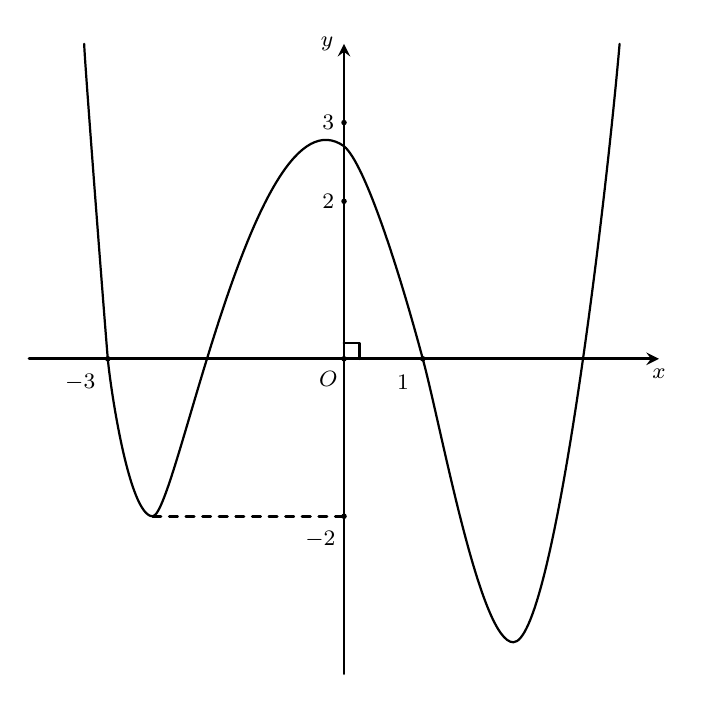
\begin{tikzpicture}[>=latex,line join=round,line cap=round,font=\footnotesize,line width=1pt,scale=1]
		\draw(0,.2)-|(.2,0);
		\draw[-stealth] (-4,0)--(4,0) node[below]{$x$};
		\draw[-stealth] (0,-4)--(0,4) node[left]{$y$};
		\coordinate (O) at (0,0);
		\coordinate (A) at (-3.3,4);
		\coordinate (Ap) at (-3,0);
		\coordinate (B) at (-2.43,-2);
		\coordinate (C) at (0,2.7);
		\coordinate (Cp) at (1,0);
		\coordinate (D) at (2.15,-3.6);
		\coordinate (E) at (3.5,4);
		\draw[thick] (A) .. controls +(270:0.15) 
		and +(95:.35) .. (Ap)
		.. controls +(275:0.35) 
		and +(180:.3) .. (B) .. controls +(0:0.3) 
		and +(145:1.4) .. (C).. controls +(320:.35) 
		and +(105:1.154) .. (Cp)
		.. controls +(285:0.95)
		and +(180:.42) .. (D) .. controls +(0:.5)
		and +(265:2.3) .. (E);
		\draw[dashed] (B)--(0,-2);
		\path[fill] (0,3) circle (1pt) +(-0.2,0) node{$ 3 $}; 
		\path[fill] (0,2) circle (1pt) +(-0.2,0) node{$ 2 $};
		\path[fill] (0,0) circle (1pt) +(-0.2,-0.25) node{$ O$};
		\path[fill] (0,-2) circle (1pt) +(-0.3,-0.3) node{$-2$};
		\path[fill] (-3,0) circle (1pt) +(-0.35,-0.3) node{$-3$};
		\path[fill] (1,0) circle (1pt) +(-0.25,-0.3) node{$1$};
		\end{tikzpicture}
	\end{center}
	Có bao nhiêu số nguyên $a$ để phương trình $f\left( \left| x^2-4x \right|-3 \right)=a$ có không ít hơn $10$ nghiệm thực phân biệt?
	\choice
	{\True $4$}
	{$6$}
	{$2$}
	{$8$}
	\loigiai{
		Đặt $t=\left| x^2-4x \right|-3$; ta có $t'\left( x \right)=\dfrac{x^2-4x}{\left| x^2-4x \right|}\cdot \left( 2x-4 \right)$.\\
		$t'\left( x \right)=0\Leftrightarrow \hoac{&x^2-4x=0 \\&2x-4=0}\Leftrightarrow \hoac{&x=0\\&x= 4 \\&x=2.}$\\
		Bảng biến thiên
		\begin{center}
			
\begin{tikzpicture}
			\tkzTabInit[ lgt=1,espcl=2.5]
			{$x$/0.7,$y'$/0.7,$y$/2}
			{$-\infty$,$0$,$ 2$,$ 4 $,$ +\infty $}
			\tkzTabLine{ ,-,d,+,0,-,d,+,}
			\tkzTabVar{+/$+\infty$,-/$-3$,+/$ 1$,-/$ -3 $,+/$+\infty$/}
			\end{tikzpicture}
		\end{center}
		Nhận thấy 
		\begin{itemize}
			\item  Với $t<-3$ thì vô nghiệm $x$.
			\item  Với $t=-3$ thì có 2 nghiệm $x$.
			\item  Với $t\in \left( -3;1 \right)$ thì có 4 nghiệm $x$.
			\item Với $t=1$ thì có 3 nghiệm $x$.
			\item Với $t>1$ thì có 2 nghiệm $x$.
		\end{itemize}
		\begin{center}
			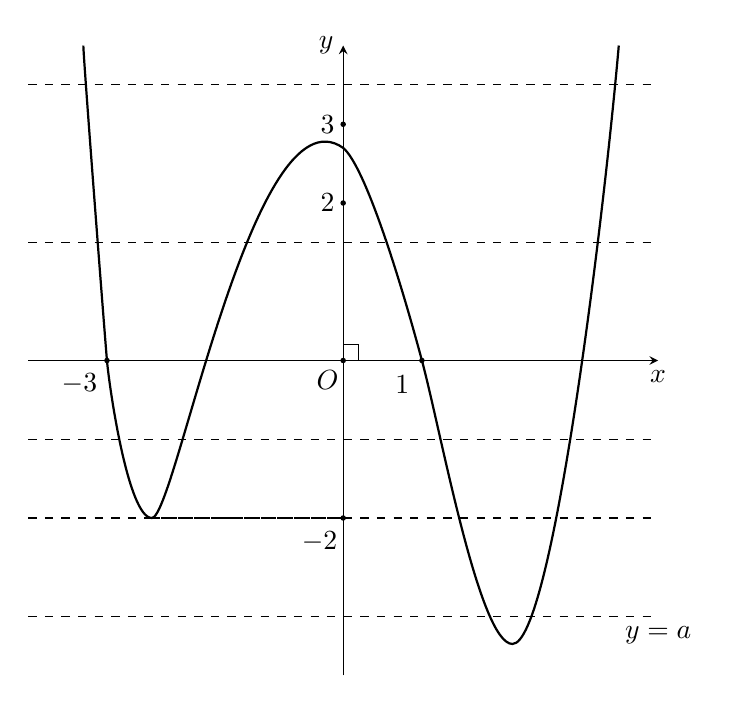
\begin{tikzpicture}
			\draw(0,.2)-|(.2,0);
			\draw[-stealth] (-4,0)--(4,0) node[below]{$x$};
			\draw[-stealth] (0,-4)--(0,4) node[left]{$y$};
			\coordinate (O) at (0,0);
			\coordinate (A) at (-3.3,4);
			\coordinate (Ap) at (-3,0);
			\coordinate (B) at (-2.43,-2);
			\coordinate (C) at (0,2.7);
			\coordinate (Cp) at (1,0);
			\coordinate (D) at (2.15,-3.6);
			\coordinate (E) at (3.5,4);
			\draw[thick] (A) .. controls +(270:0.15) 
			and +(95:.35) .. (Ap)
			.. controls +(275:0.35) 
			and +(180:.3) .. (B) .. controls +(0:0.3) 
			and +(145:1.4) .. (C).. controls +(320:.35) 
			and +(105:1.154) .. (Cp)
			.. controls +(285:0.95)
			and +(180:.42) .. (D) .. controls +(0:.5)
			and +(265:2.3) .. (E);
			\draw[dashed] (B)--(0,-2);
			\path[fill] (0,3) circle (1pt) +(-0.2,0) node{$ 3 $}; 
			\path[fill] (0,2) circle (1pt) +(-0.2,0) node{$ 2 $};
			\path[fill] (0,0) circle (1pt) +(-0.2,-0.25) node{$ O$};
			\path[fill] (0,-2) circle (1pt) +(-0.3,-0.3) node{$-2$};
			\path[fill] (-3,0) circle (1pt) +(-0.35,-0.3) node{$-3$};
			\path[fill] (1,0) circle (1pt) +(-0.25,-0.3) node{$1$};
			\draw [dashed](-4,3.5)--(4,3.5)
			(-4,1.5)--(4,1.5)
			(-4,-1)--(4,-1)
			(-4,-2)--(4,-2)
			(-4,-3.25)--(4,-3.25)node[below]{$y=a$}
			; 
			\end{tikzpicture}
		\end{center}
		Khi đó ta có phương trình $f\left( t \right)=a$ \quad (1). Từ đồ thị hàm số $f\left( x \right)$ ta có
		\begin{itemize}
			\item Nếu $a<-2$ thì (1) có 2 nghiệm phân biệt $t>1$ hoặc vô nghiệm $\Rightarrow $ Phương trình đã cho có số nghiệm không lớn hơn 4.
			\item Nếu $a=-2$ thì (1) có 3 nghiệm phân biệt trong đó 1 nghiệm $t\in \left( -3;0 \right)$ và có 2 nghiệm $t>1$ $\Rightarrow $ Phương trình đã cho có 8 nghiệm.
			\item Nếu $a\in \left( -2;0 \right)$ thì (1) có 4 nghiệm phân biệt trong đó có 2 nghiệm $t\in \left( -3;1 \right)$ và 2 nghiệm $t>1\Rightarrow $ Phương trình đã cho có 12 nghiệm phân biệt.
			\item Nếu $a=0$ thì (1) có 4 nghiệm phân biệt trong đó có 1 nghiệm $t\in \left( -3;1 \right)$ và 1 nghiệm $t>1$ và nghiệm $t=1; t=-3\Rightarrow $ Phương trình đã cho có 11 nghiệm phân biệt.
			\item Nếu $a\in \left( 0;2 \right]$ thì (1) có 4 nghiệm phân biệt trong đó có 2 nghiệm $t\in \left( -3;1 \right)$ và 1 nghiệm $t<-3$ và 1 nghiệm $t>1\Rightarrow $ Phương trình đã cho có 10 nghiệm phân biệt.
			\item Nếu $\heva{&a>2 \\&a\in \mathbb{Z}}$ thì (1) có 2 nghiệm phân biệt trong đó 1 nghiệm $t<-3$ và 1 nghiệm $t>1$ $\Rightarrow $ Phương trình đã cho có 2 nghiệm phân biệt.
		\end{itemize}
		Vậy với $-2<a\le 2$ thì phương trình đã cho có không ít hơn 10 nghiệm thực phân biệt, do đó có 4 số nguyên $a$ cần tìm.
	}
\end{ex}
\Closesolutionfile{ans}
%\inputansbox{10}{ans/ans-2-TT-ChuyenDH-Vinh-L1-NH21-22}
